\documentclass[12pt]{article}

% Package Imports
\usepackage{amsmath,amssymb}  % Math symbols
\usepackage{graphicx}         % For figures
\usepackage[margin=1in]{geometry}  % Standard margin
\usepackage{setspace}         % Adjust line spacing
\usepackage{authblk}          % For authors and affiliations
\usepackage{cite}             % For citations
\usepackage{caption}          % For figure captions
\usepackage{subfigure} 
\usepackage[numbers, sort]{natbib} % 保证参考文献不会出现乱序

% Title and Author Setup
\title{quantms and ms2rescore: deep analysis of large-scale public proteomics datasets}
\author[1,2]{Dai Chengxin}
\author[3]{Yasset Perez-Riverol}
\affil[1]{State Key Laboratory of Medical Proteomics, Beijing Proteome Research Center, National Center for Protein Sciences (Beijing), Beijing Institute of Lifeomics, 102206, Beijing, China.}
\affil[2]{International Academy of Phronesis Medicine (Guangdong), 510320, Guangdong, China.}
\affil[3]{European Molecular Biology Laboratory, European Bioinformatics Institute (EMBL-EBI), Wellcome Trust Genome Campus, Hinxton, Cambridge, CB10 1SD, UK.}
\date{}

% Document Begins
\begin{document}
\maketitle
\doublespacing  % MCP requires double-spacing

% Abstract Section
\begin{abstract}
The exponential growth of public proteomics datasets has outpaced the capacity of traditional desktop tools for large-scale automated analysis. This study presents an integrated workflow combining quantms, a cloud-native pipeline, with MS2Rescore, a machine learning-driven rescoring tool, to enable deep reanalysis of massive proteomic datasets. Leveraging the Nextflow workflow engine for parallel computing, the pipeline integrates fragment ion intensity and retention time predictions from MS2PIP and DeepLC to optimize peptide-spectrum match reliability via Percolator. Across four benchmark datasets spanning label-free quantification, TMT labeling, immunopeptidomics, and phosphoproteomics, the workflow demonstrates a 16–22.8\% increase in identified spectra compared to traditional approaches, with hundreds of newly quantified proteins and phosphosites. The results highlight that multi-search-engine collaboration with machine learning-derived features not only enhances identification sensitivity but also deepens quantitative insights for downstream biological discoveries. This approach provides a reproducible solution for large-scale reanalysis of public proteomics data, aligning with FAIR principles for scientific accessibility and reuse.

\end{abstract}

% Keywords
\noindent\textbf{Keywords:} Proteomics, Reanalysis, Workflow, Machine learning.

% Main Content
\section{Introduction}
In recent years, the field of proteomics has experienced rapid growth in the availability of publicly accessible datasets, accompanied by a shift toward studies analyzing larger sample cohorts. As of June 2025, over 40,000 datasets have been submitted to PX repositories, including a substantial increase in large-scale submissions comprising more than 100 instrument files \cite{perez-riverol_pride_2025}. However, conventional desktop tools such as MaxQuant \cite{cox_maxquant_2008}, pFind \cite{wang_pfind_2007}, MSFragger \cite{kong_msfragger_2017}, and Proteome Discoverer are limited in their capacity to perform automated, large-scale quantitative analyses in cloud or distributed environments, hindering the reanalysis of extensive experiments on standard workstations.

To address this limitation, we recently developed quantms, an open-source, cloud-based pipeline designed for massively parallel reanalysis of quantitative proteomic datasets \cite{dai_quantms_2024}. The pipeline is highly modular and flexible, accommodating a wide range of quantitative proteomics approaches. quantms automatically distributes computations using the Nextflow workflow engine across one or more computing nodes, depending on the number of instrument files and samples \cite{di_tommaso_nextflow_2017}. To ensure traceability and reproducibility, the pipeline is built entirely on standardized open file formats and reproducible execution environments, adhering strictly to the FAIR (Findability, Accessibility, Interoperability, and Reusability) principles \cite{wilkinson_fair_2016}.

With the integration of machine learning (ML) into proteomics, various models have been developed to accurately predict peptide properties, such as MS2PIP \cite{degroeve_ms2pip_2013} towards fragment ion intensities and DeepLC \cite{bouwmeester_deeplc_2021} towards retention times prediction. Early approaches employed decision trees and single-layer neural networks, while more recent deep learning models such as Prosit \cite{gessulat_prosit_2019}, achieve significantly improved accuracy for predicting fragment ion intensities and retention times. These highly accurate predictions enable superior matching of experimental data to theoretical expectations and have reinvigorated rescoring strategies in proteomics.

Previously, quantms did not leverage measurable peptide properties such as fragment ion intensities and retention times. To overcome this, we integrated MS2Rescore into quantms and incorporated customized features following Nextflow and nf-core best practices. We demonstrate that the enhanced pipeline supports in-depth analysis of large-scale public proteomics datasets across diverse experimental designs, including LFQ, TMT, immunopeptidomics, and phosphoproteomics studies.

\section{Methods}

\subsection{MS/MS Data and quantms Search Results}
To develop and evaluate the performance of quantms integrated MS2Rescore workflow, four publicly available benchmark data sets were downloaded from PRIDE Archive (29, 30) under the identifier PXD001819, PXD019463 and PXD026824 and from CPTAC under the identifier PDC000125. The PXD001819 dataset contains 48 Sigma UPS1 proteins spiked into a background of yeast cell lysate in nine different concentrations: 0.05, 0.125, 0.25, 0.5, 2.5, 5, 12.5, 25 and 50 fmol/ul to compare quantification performance. quantms enabled five different workflow settings (1) Comet, (2) Comet and MSGF+, (3)Comet with MS2Rescore, (4) Comet and MSGF+ with MS2Rescore, and (5) Comet, MSGF+ and SAGE with MS2Rescoring to explore multiple search engines and integrate with MS2Rescore for improved identification and quantification results. All search parameters were the same as described in the previous publication. The quantms and MaxQuant search results on PSM and protein group level of this search are also available in parquet format in supplemental File S1.


\subsection{Rescoring feature and Postprocessing}
Search engines features are generated in OpenMS toolkit. quantms-rescoring python package integrated MS2Rescore and calculates various meaningful features based on the DeepLC-predicted and the observed retention times, and the MS2PIP-predicted and the observed MS2 peak intensities. SNR features are also calculated for specific cases in quantms-rescoring python package. Percolator module was subsequently used to rescore the common pool of PSMs for different feature combinations in different strategies: (1) a baseline setting with only the search engine features (2) the baseline setting combined with the features from MS2Rescore, and (3) the baseline setting combined with the features from MS2Rescore and quantmsutils package. 


\section{Results}

\subsection{quantms with MS2Rescore enchancing identification and quantification in label free experiments}
To systematic evaluation the performance of quantms integrated MS2Rescore on identification and quantification level,  we firstly collected a public benchmark datasets PXD001819. For identification benchmark analysis, five different identification workflow and designed and compared, including (1) Comet with Percolator, (2) two search engines with Percolator, (3) Comet with MS2Rescore features and Percolator, (4) two search engines with MS2Rescore features and Percolator and (5) three search engines with MS2Rescore features and Percolator to check whether the features added by the intensity-based and RT-based predictors features boosted the identification and quantification process.

Filtering for a set of significant PSMs is generally performed using the q-values and the resulting FDR-estimation (18). The most valuable measure to compare the sets with and without additional features is therefore the FDR as this shows the actual yield on PSM-level stringency. In Figure ~\ref{fig:PXD001819_ms2rescore_pic}, it is clearly visible that the 
two search engines consensus score extensively improve identification rate in same FDR level. The multiple search engines consensus score improved the number of spectra identified by 17\% compared with the Comet identification. The number of spectra identified increased by a further 16\% after adding MS2PIP and DeepLC features. Feature calculation is done using the standalone MS2ReScore tool. We further explore the effect of different settings on protein quantification results especially for adding extra features. More low abundance USP1 proteins are quantified after adding MS2Rescore features (Figure 2B).

Moreover, we extracted the top 20 weights of Percolator to explore the impact of different features on rescoring for different search engines, shown as Supp Figure 1. We can see that more than half of the features are from the MS2Rescore, and distribution of features are different for three search engines. The weight of SpecPearsonNorm is positive that indicates of a high SpecPearsonNorm gives a better hit. The weight of the RtDiffBest is negative, which indicates that large differences between observed and predicted RT gives a worse score. It is interesting that peptide length becomes a significant feature after adding MS2Rescore features. The positive value demonstrates that higher scores for longer peptides. One potential explanation for this phenomenon is that short peptides are less conducive to search engine identification due to fewer fragment ions. 

% Figure Example
\begin{figure}[h!]
	\centering
	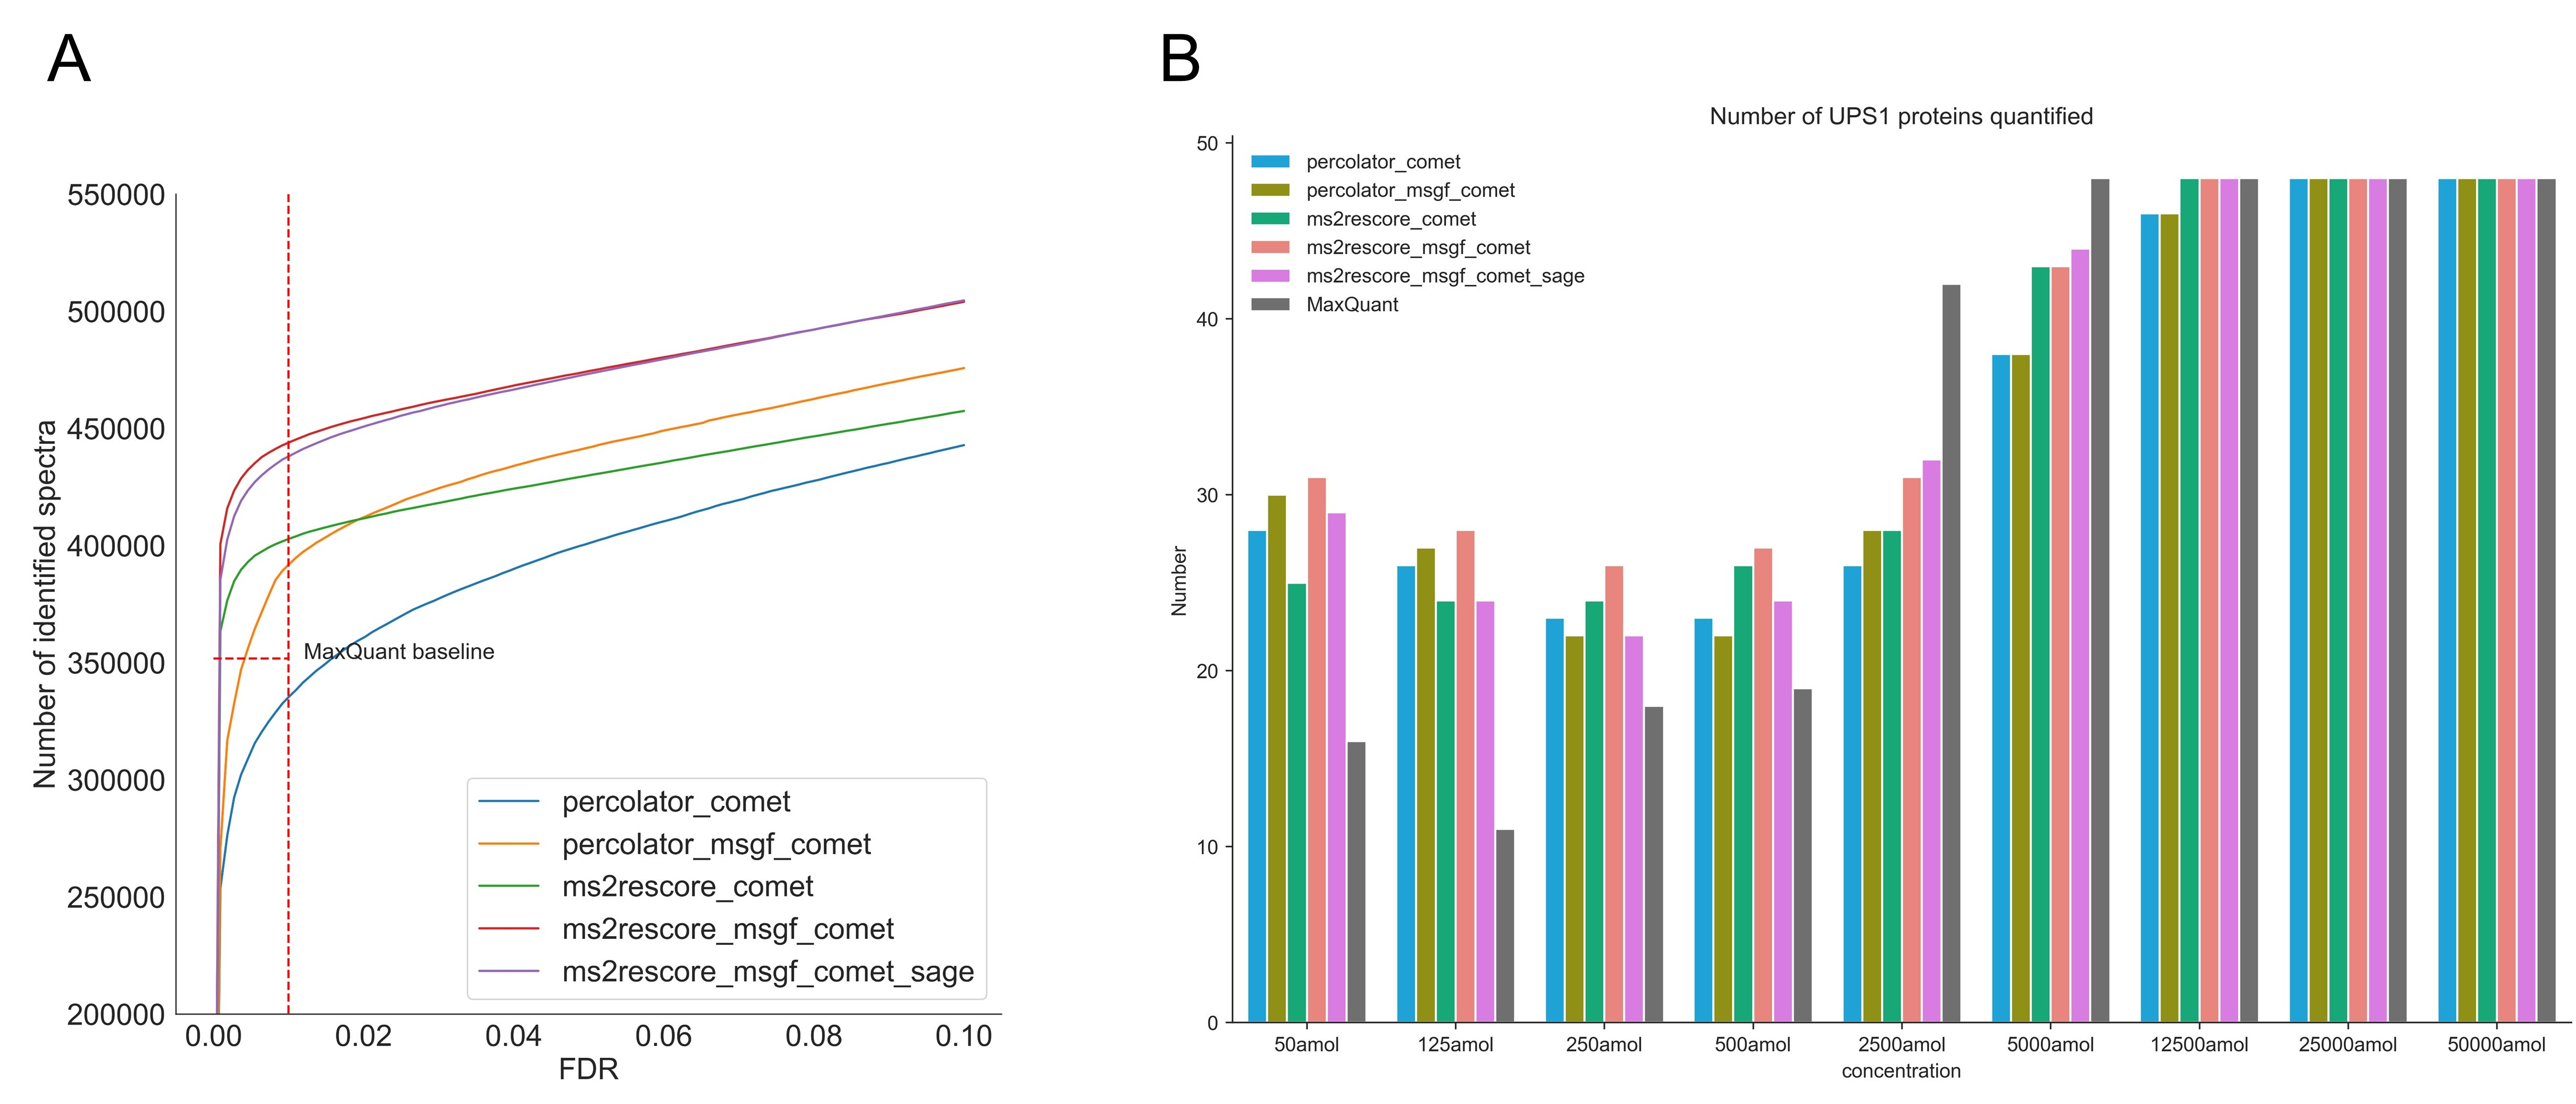
\includegraphics[width=1\textwidth]{figures//PXD001819.jpg}
	\caption{The number of identified spectra as a function of differing FDR levels for the different workflow setting. A, for the PXD001819 datasets. B, for the PXD014415 datasets. Five different workflow setting, the combination of Comet search engine with Percolator rescore, the combination of Comet with MSGF+, the combination of two search engines with MS2ReScore features, and the combination of two search engines with MS2ReScore and SNR features, and the combination of three search engines with MS2ReScore and SNR features are shown. Multiple search engines consensus identification, additional intensity-based, retention time-based features, and SNR features leading to both a higher identification rate as well as an high quality identification.}
	\label{fig:PXD001819_ms2rescore_pic}
\end{figure}


\subsection{quantms integrated MS2Rescore drastically improves identification and quantifications for large-scale TMT experiments}
Then we applied this workflow to large-scale TMT experiments from CPTAC. Multiple search engines and rescoring significantly improved peptide identification and protein quantification, as shown in Fig~\ref{fig:PDC_ms2rescore}. PSM identification rate was improved by 3.6\% and 921 proteins were newly quantified when deeplc and MS2PIP features were added, compared to the workflow without ms2rescore enabled (Figure 2A,B). There are 59 newly quantified to proteins whose abundance is located in the top 10\% (Figure 2C). To further explore the impact of these newly quantified proteins from the two search engines with MS2Rescore features workflow on downstream analysis, protein differential expression results from this workflow are shown in Figure 2. There are 27 newly quantified proteins that are significantly differentially expressed (Figure 2D). Among them, Yang et al. reported an association between significant upregulation of FOXG1 protein and prognosis in Clear Cell Renal Cell Carcinoma [10.18632/aging.204448]. This further illustrates that by incorporating re-scoring features based on ms2pip and deeplc, it not only improves the sensitivity of spectral identification, but also facilitates the quantification of proteins, which ultimately contributes to the discovery of biological knowledge. 

Moreover, we extracted the top20 SVM weights of Percolator to explore the impact of different features on rescoring for different search engines, shown as Supp Figure ~\ref{fig:PDC_ms2rescore_weights}. For Comet identification results, SpecPearsonNorm, DotProdIonYNorm and RtDiffBest features have significant weights for final rescoring. The weight of SpecPearsonNorm is positive that indicates of a high SpecPearsonNorm value between MS2PIP prediction and experimental intensities gives a better hit. The weight of the RtDiffBest is negative, which indicates that large differences between observed and calculated retention time gives a worse score. It is interesting that peptide length becomes a significant feature after adding MS2Rescore features. The positive value demonstrates that higher scores for longer peptides. One potential explanation for this phenomenon is that short peptides are less conducive to search engine identification due to fewer fragment ions. For other two search engines, similar distribution of weights can be observed. SpecPearsonNorm, DotProdIonYNorm and RtDiffBest features still have significant weights.


% Figure Example
\begin{figure}[h!]
	\centering
	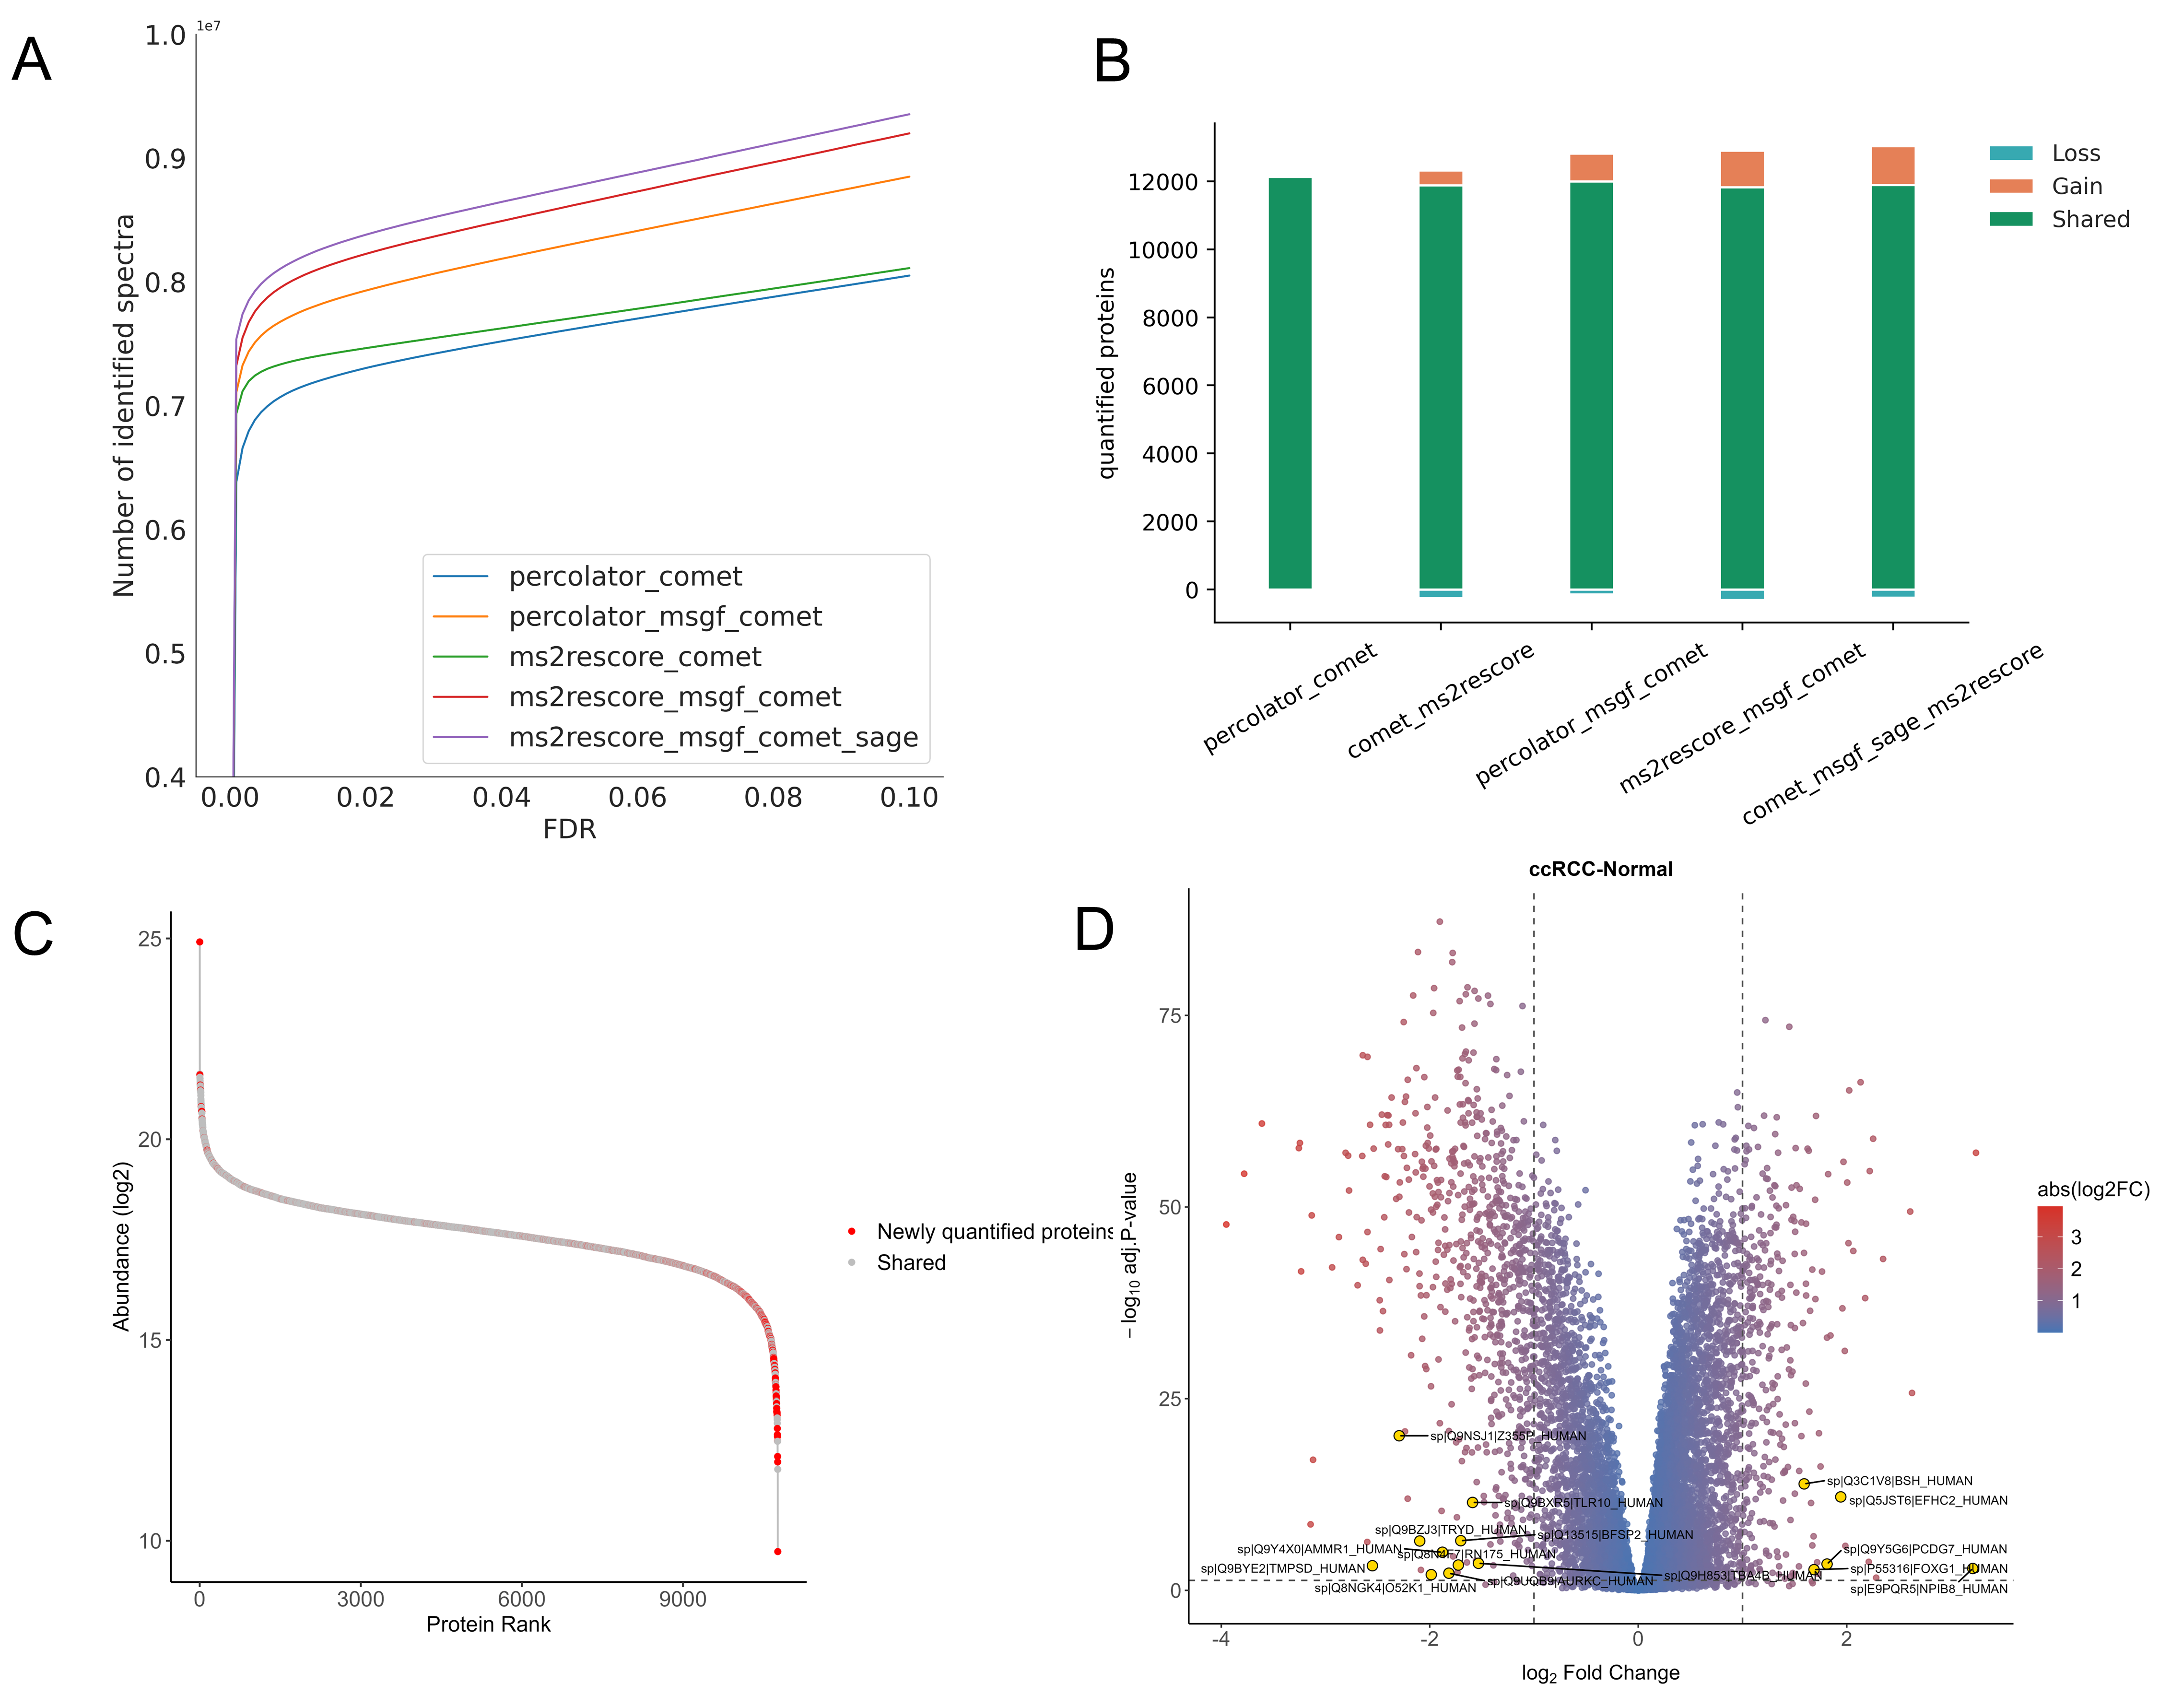
\includegraphics[width=1\textwidth]{figures//CPTAC_TMT.png}
	\caption{The comparison of identification and quantification results for the different workflow setting. A, the number of identified spectra as a function of differing FDR levels for the different workflow setting. B, the number of quantified proteins. The green part indicates the intersection between a workflow and Comet results. C, the rank of protein abundance from Comet and MSGF+ with MS2Rescore. The red dots represent proteins quantified only in Comet and MSGF+ with MS2Rescore workflow compared to Comet and MSGF+ workflow without MS2Rescore. D, the volcano plot for differential expression analysis from MSstatsTMT. The red dots represent proteins quantified only in Comet and MSGF+ with MS2Rescore workflow compared to Comet and MSGF+ workflow without MS2Rescore.}
	\label{fig:PDC_ms2rescore}
\end{figure}


\subsection{Evaluation of quantms integrated MS2Rescore on HLA Class I Peptides}
Further, we evaluated the performance of quantms identification workflow in immunopeptides datasets PXD019643. Therefore, four different workflow setting the combination of Comet search engine with Percolator rescore, the combination of Comet with MSGF+, the combination of two search engines with MS2ReScore features, and the combination of two search engines with MS2ReScore and SNR features were compared in terms of the total amount of identifications as well as the number of unique identifications based on sequence. Overall, multiple search engines and rescoring with both MS2Rescore substantially improved the spectrum identification rate in comparison with only Comet search engine or not rescoring at both 1\% and 0.1\% FDR. Multiple search engines achieves the number of spectra identified by an increase of  11.7\% compared to only Comet search engines, and then MS2Rescore features further achieved the number of spectra identified by an increased 22.8\% compared to multiple search engines without MS2Rescore features, shown as Figure ~\ref{fig:PXD019643_immunopeptides}.

The power of providing these predictions to Percolator is further illustrated when visualizing the distributions for decoy PSMs, rejected target PSMs, and accepted target PSMs from individual support and from consensus supports (Figure 3C, D). The accepted target PSMs are clearly separable from the decoy and rejected target PSMs using only the PCC. And the distributions for accepted targets from individual support and consensus supports are highly similar in that they both lie around low retention time errors and high PCC. This further demonstrates that quantms is reasonable for integrating the identification scores of multiple search engines. 

% Figure Example
\begin{figure}[h!]
	\centering
	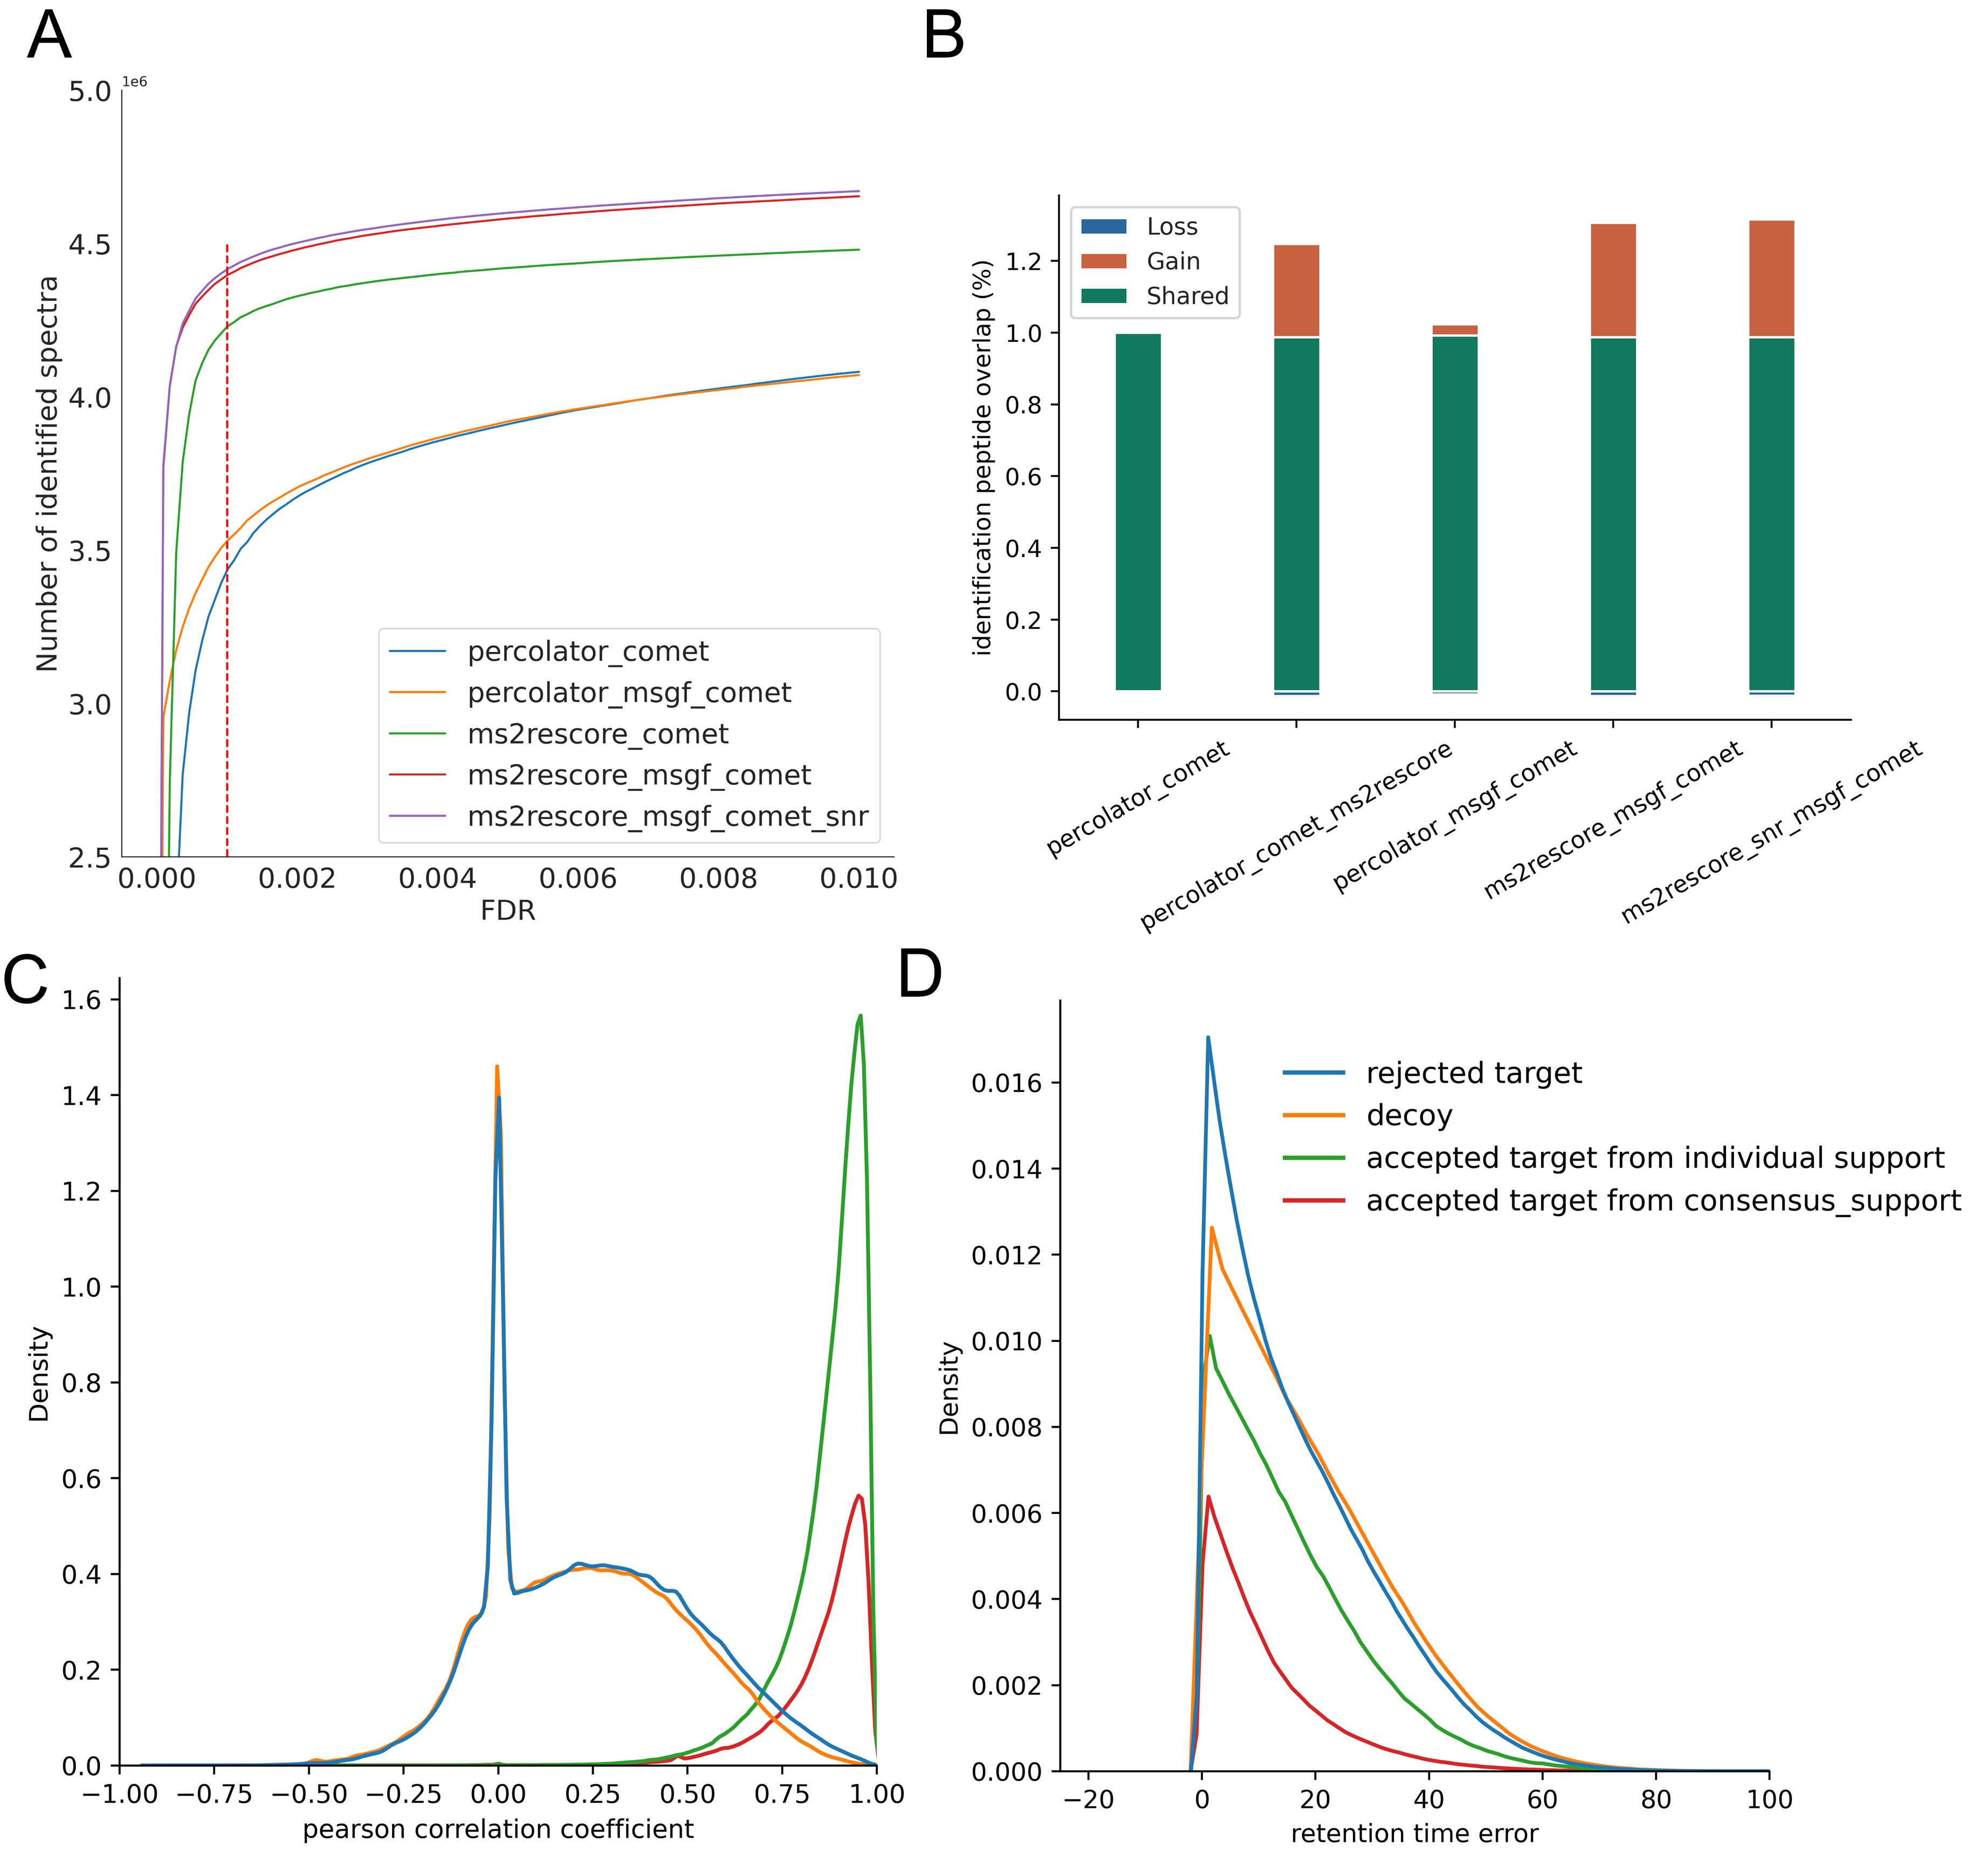
\includegraphics[width=1\textwidth]{figures//PXD019643.png}
	\caption{Comparison of the immunopeptides identification results for five workflow setting. A, Line plot showing the number of spectra identified for four workflow setting at different PSM FDR level. B, Percentage of unique identified peptides using different workflow setting. Density plots showing the distribution of the smallest retention time error between observed and predicted retention time (C) and showing the Pearson correlation between observed and predicted peak intensities (D) for each PSM split in decoys (red) rejected targets, q value >0.01(blue) and accepted targets from individual support and consensus support, q value <0.01 (green) (note the rejected targets distribution coincides with the decoy distribution).}
	\label{fig:PXD019643_immunopeptides}
\end{figure}


\subsection{quantms integrated MS2Rescore facilitates the identification of phosphorylated peptides}
In addition, we also investigated the yield of our quantms workflow with MS2Rescore on the post-translational modifications experiments (PXD026824). For the case of Phospho analyses, different workflow setting for (1) Comet alone, (2) Comet combined with MSGF+, and (3) multiple search engines combined with MS2Rescore features were processed using Percolator to check whether multiple search engines and M2Rescore facilitated the identification and quantification process. In Figure ~\ref{fig:PXD026824_ms2rescore}, it is clearly visible that the introduced multiple search engines consensus identification and MS2ReScore features extensively improve the stringency on which Percolator can classify the PSMs. This is illustrated by the remarkable shift to the left, compared with the Comet only. Next to that, there is also a gain in identification rate, which is shown in the vertical direction of this figure. The two search engines consensus identification combined with MS2Rescore features enabled the number of spectra identified increased by 19\% compared to consensus identification without MS2Rescore (Figure 4A). The top 20 weights of Percolator is shown as supplemental Fig.  ~\ref{fig:phospho_features}.  We can observe same features as above results, such as DotProdIonYNorm feature.

Protein phosphosite false localization rate (FLR) control is necessary for Phosphoproteomics analysis. Therefore, we also investigate the effect of different workflow settings on phosphorylated peptides at different FLR level (Fig. 7B, C). The search engines consensus identification combined with MS2Rescore features increased the number of phosphorylated peptide identifications by 17\% at 0.01 local FLR compared to without MS2Rescore. Then there are 1345 phosphorylated peptides quantified only in consensus identification combined with MS2Rescore process. Considering protein phosphosites, consensus identification combined with the MS2Rescore process newly reports 350 protein phosphorylation sites (Fig 7D). Altogether, these results show that quantms integrated MS2Rescore can boost the performance on phosphoproteomics.



% Figure Example
\begin{figure}[h!]
	\centering
	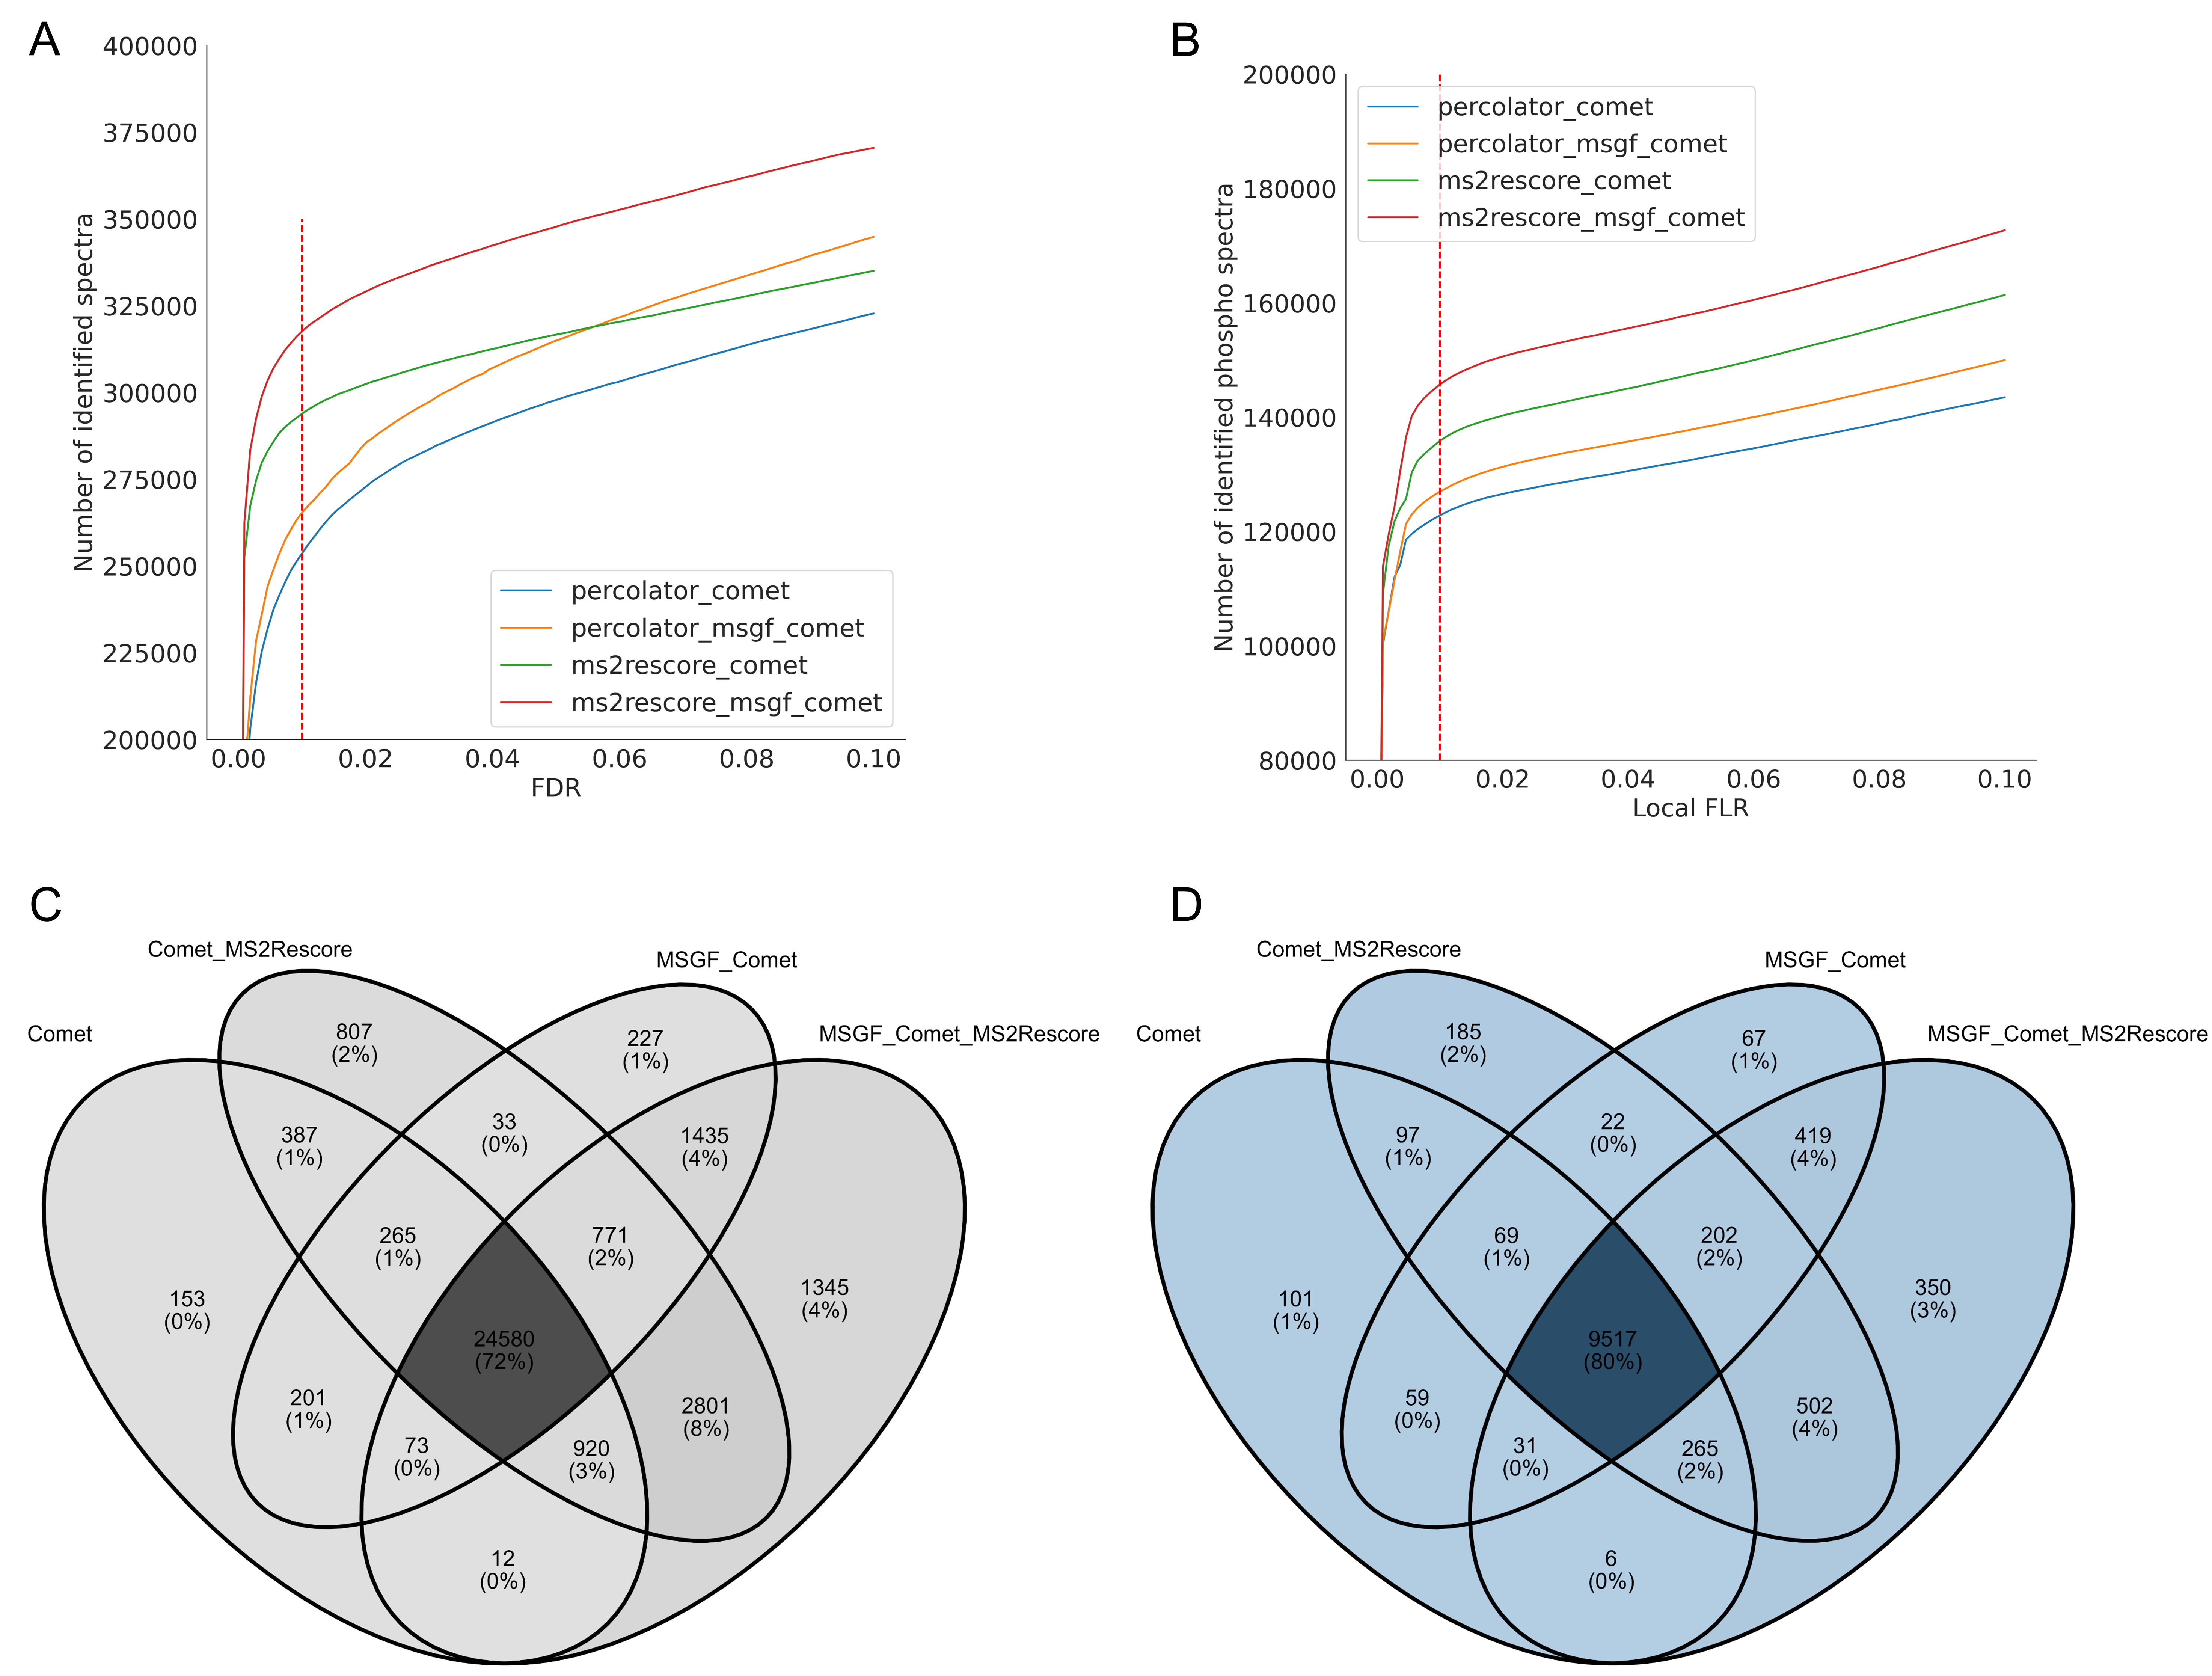
\includegraphics[width=1\textwidth]{figures//phospho2.png}
	\caption{Comparison of the phosphorylated peptide identification results for five workflow setting. A, line plot showing the number of spectra identified for four workflow setting at different PSM FDR level. B, line plot showing the number of phosphorylated spectra identified for four workflow setting at different local false localization rate level after an FDR of less than 0.01 at the PSM level. C, the Venn plot of peptides quantified for four settings. D, the Venn plot of protein phosphosites at protein fdr 0.01 and FLR 0.01 for four setting.}
	\label{fig:PXD026824_ms2rescore}
\end{figure}


\section{Discussion}
Advancements in deep learning–based tools have significantly improved the accuracy and sensitivity of peptide-spectrum match (PSM) rescoring, yet their integration into streamlined, reproducible, and quantitative proteomics workflows has remained limited, especially for large-scale public data analysis. In this study, we demonstrate the systematic incorporation of MS2Rescore into the open-source quantms pipeline and evaluate its impact across various experimental settings, including label-free quantification (LFQ), tandem mass tag (TMT)-based quantification, immunopeptidomics, and phosphoproteomics. Our results show that enhanced feature sets derived from MS2PIP and DeepLC not only improve identification rates, but also translate into gains in quantification depth. Importantly, we provide evidence that the improved identifications via rescoring propagate downstream into quantification, leading to increased numbers of proteins with reliable abundance estimates, as well as enhanced detection of differentially expressed proteins.

In order to demonstrate the applicability and the advantages of quantms integrated MS2Rescore in quantitative proteomics, we performed a series of reanalyses using publicly available large-scale datasets with well-established benchmarks. In label-free experiments, MS2Rescore-enhanced workflows achieved significant increases in PSM and peptide identification while maintaining or improving quantification reproducibility across replicates. For TMT experiments, the integration of MS2Rescore into quantms increased the number of quantifiable proteins. In more challenging applications, such as immunopeptidomics and phosphoproteomics, the deep learning–based rescoring pipeline consistently yielded higher identifications and improved. These improvements contribute meaningful biological insights such phosphosites discovery.

Overall, the results in this publication highlight the synergistic benefits of integrating machine learning–based features within end-to-end, cloud-based proteomics workflows. By embedding MS2Rescore into the quantms pipeline, we provide a practical and accessible solution for the community to leverage cutting-edge spectral prediction and retention time modeling without the need for complex manual configuration. This integrated approach enables reproducible reanalysis of large public datasets, increases identification confidence, and strengthens quantitative conclusions across diverse experimental designs.



In order to demonstrate the applicability and the advantages of these new machine learning–based PSM rescoring techniques in proteogenomics,


Over all the results in this publication,


\section*{Acknowledgments}
Thank those who supported the research, including funding bodies.

% References Section
\bibliographystyle{abbrv}  % Abbreviated style similar to MCP
\bibliographystyle{unsrt}
\bibliography{references}  % references.bib file contains your bibliography


\renewcommand\thefigure{S\arabic{figure}}
\setcounter{figure}{0}

% Figure Example
\begin{figure}[h!]
	\centering
	\includegraphics[width=1\textwidth]{figures//LFQ_weights.png}
	\caption{The weights that Percolator appoints to the different features of the search engine feature vector in the MSGF+ (A), Comet (B) and Sage (C) combined with Percolator setting from PXD001819. The more different from zero a weight is (both positive and negative), the more important that feature is in the final Percolator classification.}
	\label{fig:PXD001819_svm_weights}
\end{figure}

% Figure Example
\begin{figure}[h!]
	\centering
	\includegraphics[width=1\textwidth]{figures//CPTAC_weights.png}
	\caption{The top 20 normalized weight of Percolator for MSGF (A), for Comet (B) and for Sage (C) identification results from PDC000120.}
	\label{fig:PDC_ms2rescore_weights}
\end{figure}


\begin{figure}[h!]
	\centering
	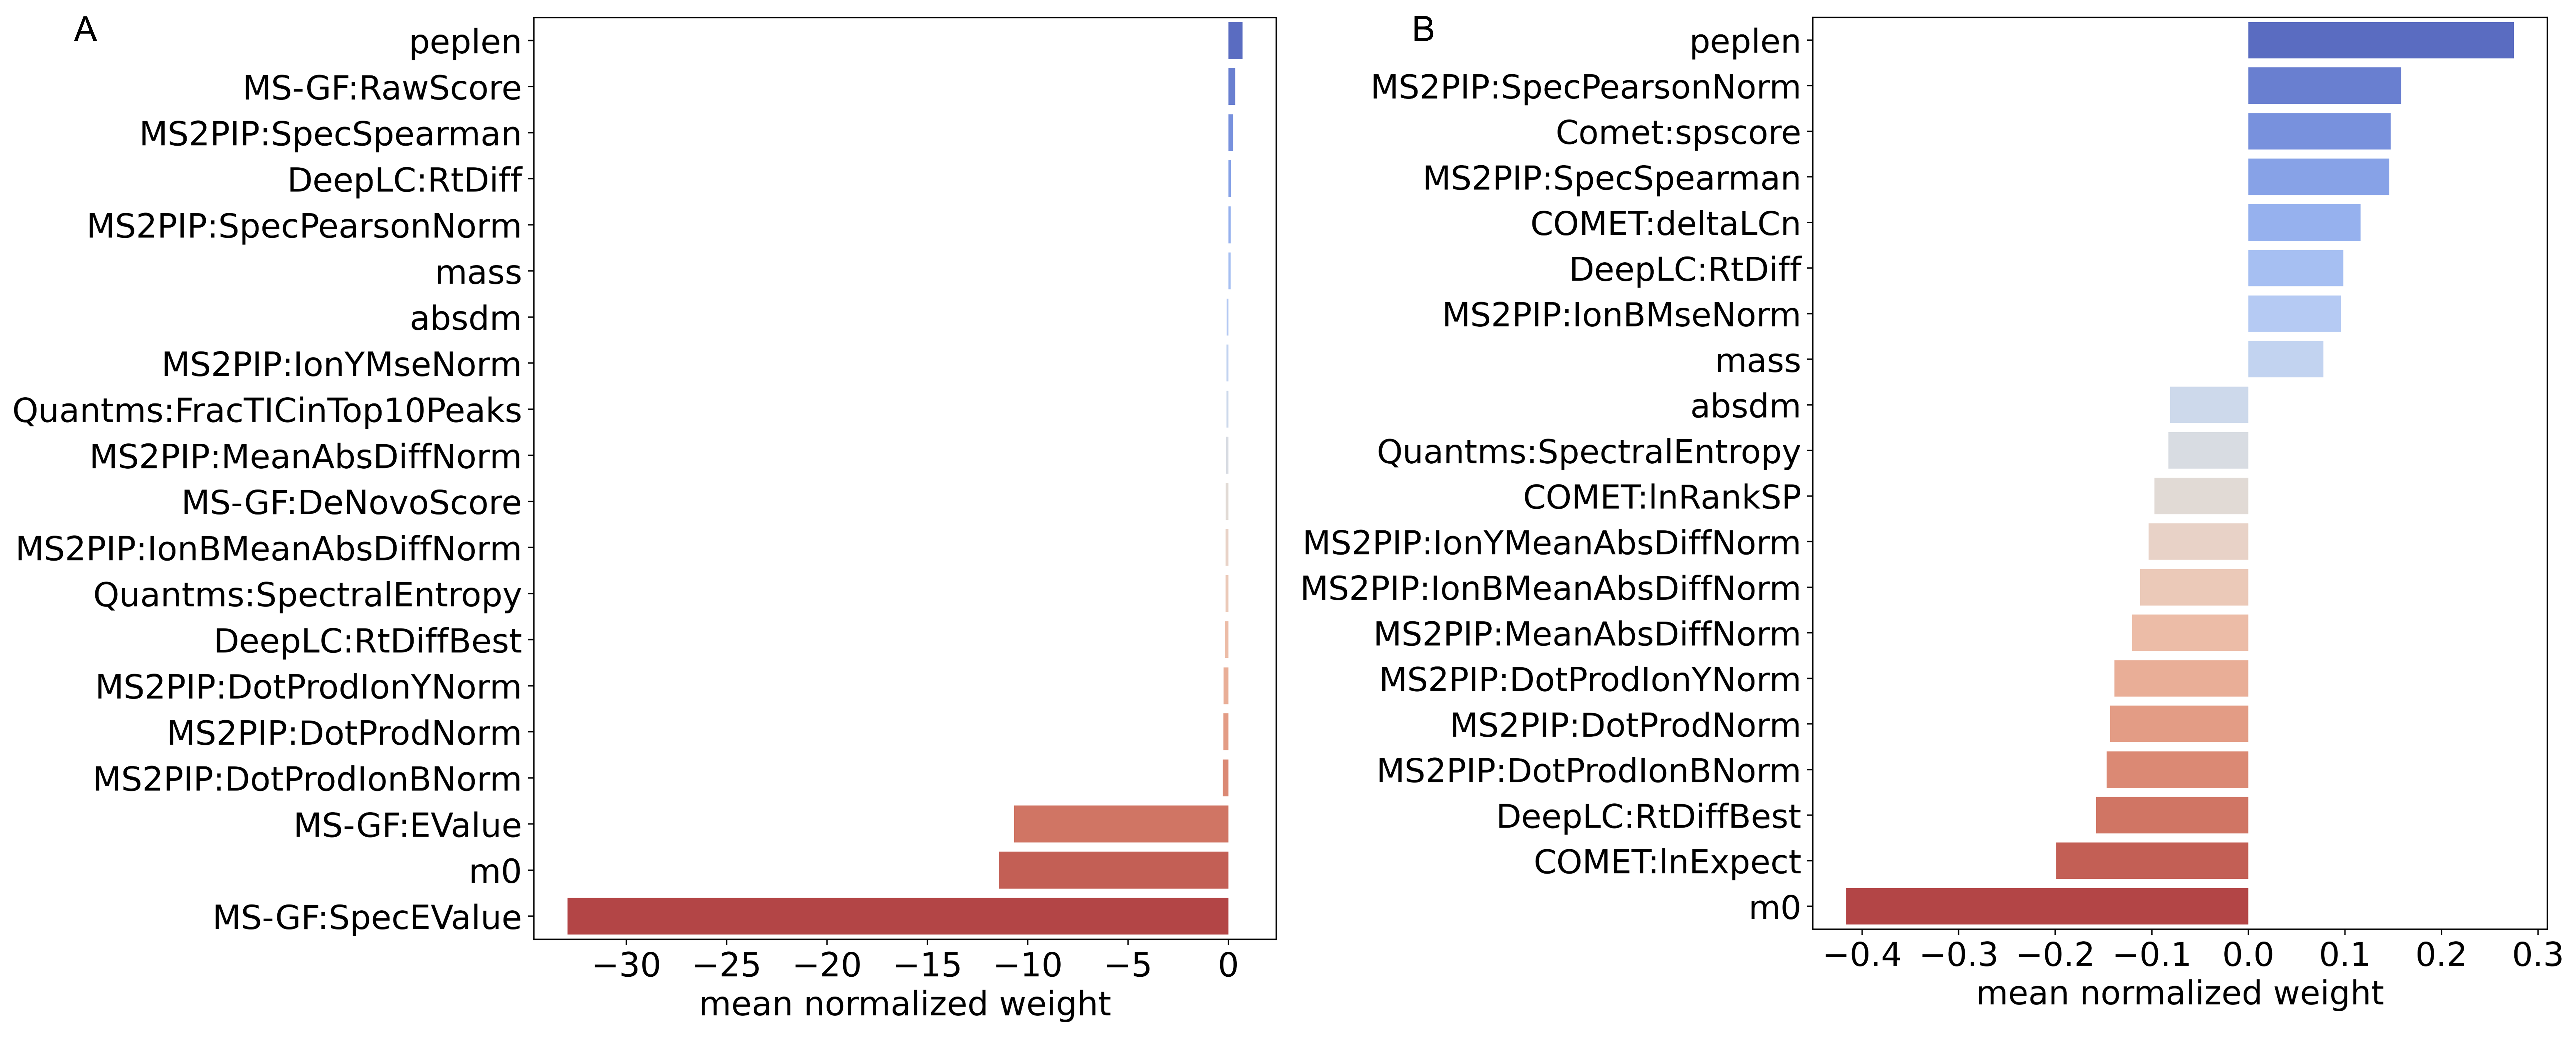
\includegraphics[width=1\textwidth]{figures//PXD019643_weights.png}
	\caption{The top 20 normalized weight of Percolator for MSGF (A) and Comet (B) identification results in PXD019643 dataset.}
	\label{fig:PXD019643_features}
\end{figure}

\begin{figure}[h!]
	\centering
	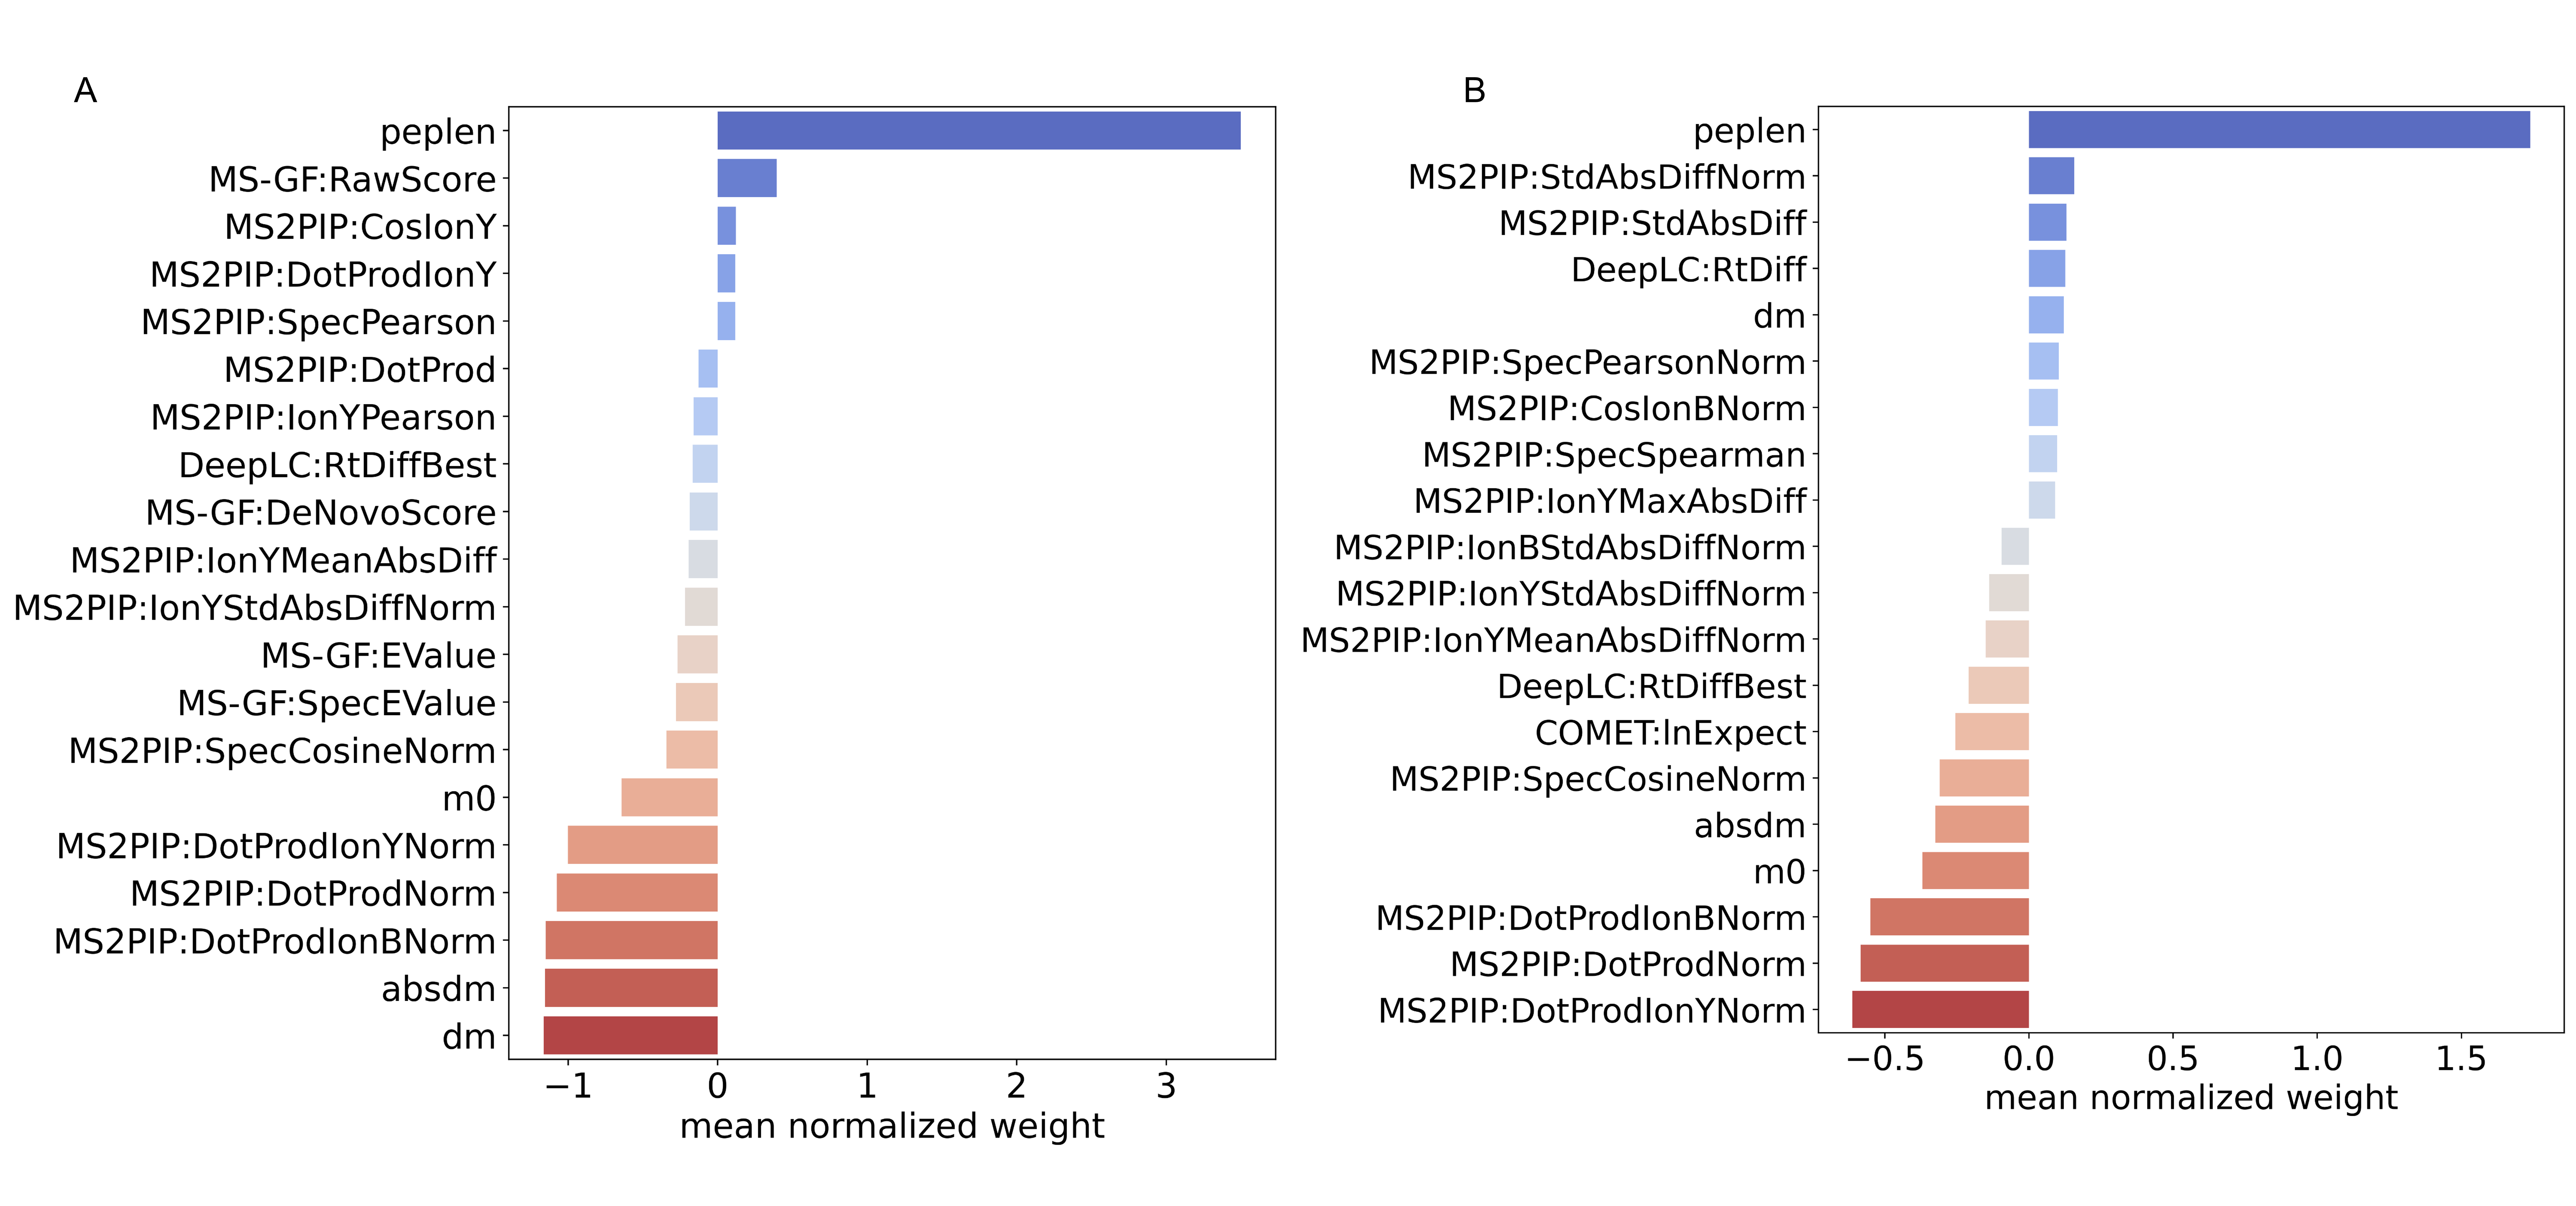
\includegraphics[width=1\textwidth]{figures//phos_weights.png}
	\caption{The top 20 normalized weight of Percolator for MSGF (A) and Comet (B) identification results in PXD026824 dataset.}
	\label{fig:phospho_features}
\end{figure}


\end{document}

